\section{Кратные интегралы}

\subsection{Множества, измеримые по Жордану}

\begin{definition}
    Пусть множество 
    $A = \{ (x_1, \dots, x_n): a_i \leq x_i \leq a_i + h_i, i = \overline{1, n} \}
    \quad (a_i, h_i \text{ --- const})$ $m$-мерный прямоугольный параллелепипед
    (рёбра параллельны оси $X$-координат).

    Назовём его мерой число $mA = \ds\prod_{i = 1}^m h_i$.
    Если $h_i = h, \, i = \overline{1, m}$, то $A$ --- 
    $m$-мерный куб и $mA = h^m$.
\end{definition}

\begin{definition}
    Пусть множество $B$ составлено из прямоугольных параллелепипедов
    $A_j (j = \overline{1, n})$, пересекающихся разве что по части границ.
    Тогда $B$ назовём элементарной фигурой и определим меру $B$ как 
    $mB = \ds\sum_{j = 1}^n m A_j$

    Мерой пустого множества будем считать 0.
\end{definition}

\begin{remark}
    Очевидны свойства мер элементарных фигур:

    \begin{enumerate}
        \item $B_1 \subset B_2 \implies mB_1 \leq mB_2$
        \item
            Объединение элементарных фигур является элементарной фигурой и её
            мера не превосходит суммы мер этих фигур, причём равенство будет
            только в том случае, если эти фигуры пересекаются разве что по
            части границ.
        \item
            Если элементарную фигуру $B$ рассечь плоскостью $X_i = const$, то
            она разделится на две элементарные фигуры $B'$ и $B''$, причём
            $mB = mB' + mB''$
    \end{enumerate}
\end{remark}

\begin{definition}
    Рассмотрим в пространстве $\R^m$ сеть кубов
    \[ k_i h \leq x_i \leq (k_i + 1) h \]
    где $k_i = 0; \pm 1; \pm 2; \dots$. $h = \frac{1}{2^N}$, $N$ --- натуральное
    число.

    При увеличении $N$ на 1 каждый куб прежней сети делится на $2^m$ кубов.
    Пусть $A$ --- ограниченное множество в пространстве $\R^m$. Рассмотрим
    $\underline{A_N}$ --- элементарную фигуру, состоящую из кубов сети, которые
    состоят из внутренних точек множества $A$ и
    $\overline{A_N}$ --- элементарную фигуру, состоящую из кубов сети,
    имеющих с $A$ хотя бы одну общую точку.

    \begin{figure}[H]
        \centering
        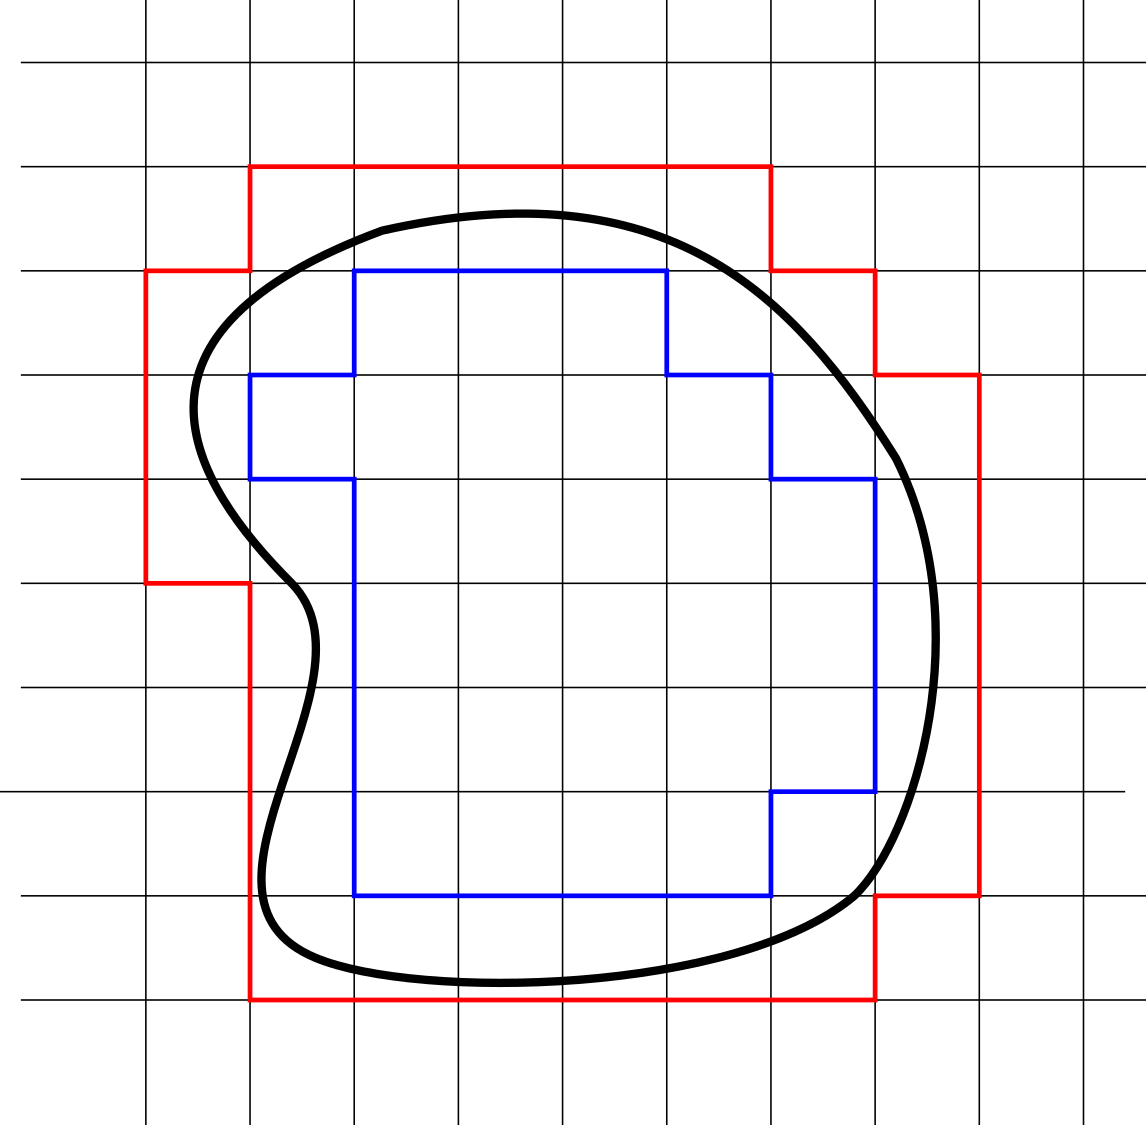
\includegraphics[width=0.3\textwidth]{images/multiple_border.png}
    \end{figure}

    При увеличении $N$ на 1 $m \underline{A_N}$ может только неубывать, а 
    $m \overline{A_N}$ только невозрастать и $\{ m \underline{A_N} \}$ 
    ограничена сверху (любой $m \overline{A_{N_0}}$) и $\{ m \overline{A_N} \}$ 
    ограничена сверху (любой $m \underline{A_{N_0}}$) $\implies$ (так как 
    ограниченная монотонная последовательность сходится)

    \begin{align*}
        \exists \ds\lim_{N \to \infty} \underline{A_N} = m_i A \; \text{--- внутренняя мера} \; A    
        \exists \ds\lim_{N \to \infty} \overline{A_N} = m_e A \; \text{--- внешняя мера} \; A    
    \end{align*}

    Если внутренняя мера $A = $ внешней мере $A$, то множество $A$ назовём
    измеримым по Жордану и $m_i A = m_e A = mA$ назовём мерой $A$ по Жордану.
\end{definition}

\begin{remark}
    Очевидные свойства измеримого множества:

    \begin{enumerate}
        \item Любое измеримое множество ограничено.
        \item
            Мера границы $\overline{\Gamma_N}$ измеримого множества $= 0$ 
            (Граница --- граничной точкой множества $A$ называется точка, в 
            любой окрестности которой есть точки как принадлежащие множеству
            $A$, так и не принадлежащие ему. Множество граничных точек 
            множества $A$ называется \textbf{границей} $A$).
    \end{enumerate}
\end{remark}

\begin{theorem}
    Для того, чтобы ограниченное множество $A$ было измеримым $\iff$ чтобы
    мера его границы была равна 0.

    $\forall N \quad m \overline{A_N} = m \underline{A_N} + m \overline{\Gamma_N}$,
    где $\Gamma$ --- граница $A$.
\end{theorem}
\begin{proof}
    \begin{enumerate}
        \item 
            $A$ --- измеримо $\implies 
            \ds\lim_{N \to \infty} m \underline{A_N} = 
            \ds\lim_{N \to \infty} m \overline{A_N} \implies
            \ds\lim_{N \to \infty} m \overline{\Gamma_N} = 0$ и так как
            \[ 
                0 \leq m \underline{\Gamma_N} \leq m \overline{\Gamma_N} 
                \implies m\Gamma = 0 
            \]
        \item
            $\Gamma$ --- измерима и $m\Gamma = 0 \implies 
            \underbrace{\ds\lim_{N \to \infty} m \overline{\Gamma_N}}_{m_e \Gamma} = 0$

            $\implies \ds\lim_{N \to \infty} m \overline{A_N} = 
            \ds\lim_{N \to \infty} \underline{A_N} + 0
            \implies m_e A = m_i A \implies A$ --- измеримое.
    \end{enumerate}
\end{proof}